
\section{Computation and Empirical Evaluation}

We have two modified VAE loss (Eq. \ref{eq:unsup_objective}) and modified VIB loss (Eq. \ref{eq:sup_objective}).
In both we have to learn an encoder and decoder pair $q(z|x)$ and $p(x|z,c)$. We use feed forward networks to approximate these functions. For $q(z|x)$ we use the Gaussian reparameterization trick, and for $p(x|z,c)$ we simply concatenate $c$ onto $z$ as extra input features to be decoded. In the modified VIB we also have a predictor branch $p(y|z)$, which we also use a feed forward network to parametrize. Specific architectures (e.g. number of layers and nodes per layer for each branch) vary by domain.

%In order to empirically evaluate our proposed invariance penalty, we implemented and experimented on the modified VAE and VIB from Section \ref{subsec:vae} and \ref{subsec:sup}.
We evaluate the performance on of our proposed invariance penalty on two datasets with a ``fair classification'' task. We also demonstrate ``Fader Network''-like capabilities for manipulating specified factors in generative modeling on the MNIST dataset.

\subsection{Fair Classification}

For each fair classification dataset/task we evaluated both prediction accuracy and adversarial error in predicting $c$ from the latent code. We compare against the Variational Fair Autoencoder (VFAE) \cite{louizos2015variational}, and the adversarial method proposed in Xie et al. \cite{xie2017controllable}. Both datasets are from the UCI repository. The preprocessing for both datasets follow Zemel et al. 2013\cite{zemel2013learning}, which is also the source for the pre-processing in our baselines \cite{louizos2015variational,xie2017controllable}.

The first dataset is the German dataset, containing 1000 samples of personal financial data. The objective is to predict whether a person has a good credit score, and the protected class is Age (which, as per \cite{zemel2013learning}, is binarized). The second dataset is the Adult dataset, containing 45,222 data points of US census data. The objective is to predict whether or not a person has over 50,000 dollars saved in the bank. The protected factor for the Adult dataset is Gender\footnote{In some papers the protected factor for the Adult dataset is reported as Age, but those papers also reference Zemel et al. \cite{zemel2013learning} as the processing and experimental scheme, which specifies Gender.}.

Wherever possible we use architectural constraints from previous papers. All encoders and decoders are single layer, as specified by  Louizos et al. \cite{louizos2015variational} (including those in the baselines), and for both datasets we use 64 hidden units in our method as in Xie et al., while for VFAE we use their described architecture. We use a latent space of 30 dimensions for each case. We train using Adam using the same hyperparameter settings as in Xie et al., and a batch size of 128. Optimization and parameter tuning is done via a held-out validation set.

For each tested method we train a discriminator to predict $c$ from generated latent codes $z$. These discriminators are trained independently from the encoder/decoder/within-method adversaries. We use the architecture from Xie et al. \cite{xie2017controllable} for these post-hoc adversaries, which describes a three-layer feed-forward network trained using batch normalization and Adam (using $\gamma = 1$ and a learning rate of $0.001$), with 64 hidden units per layer, using absolute error. We generalize this to four adversaries, increasing in the number of hidden layers. Each discriminator is trained post-hoc for each model, even in cases with a discriminator in the model (e.g. the model proposed by Xie et al. \cite{xie2017controllable}).

\subsection{Unsupervised Learning}

We demonstrate a form of unsupervised image manipulation inspired by Fader Networks \cite{lample2017fader} on the MNIST dataset. We use the digit label as the covariate class $c$, which pushes all non-class stylistic information into the latent space while attempting to remove information about the exact digit being written. This allows us to manipulate the decoder at test time to produce different artificial digits based on the style of one digit. We use 2 hidden layers with 512 nodes for both the encoder and the decoder.

\section{Results}

% \begin{table}[h!]\centering
% \begin{tabular}{ | l | l | l | l | l |}
% \hline
% Predictive Acc. & VFAE & Xie et al. & Proposed \\\hline
% German Dataset & 0.693 & 0.710 & 0.695 \\\hline
% Adult Dataset & 0.751 & 0.845 & 0.752\\\hline 
% \end{tabular}

% \begin{tabular}{ | l | l | l | l | l |}
% \hline
% Adversarial Loss & VFAE & Xie et al. & Proposed \\\hline
% German Dataset & 0.948 & 0.992 & 0.81 \\\hline
% Adult Dataset & 0.983 & 0.986 & 0.681\\\hline 
% \end{tabular}
% \end{table}

\begin{figure}[t]
\begin{center}
\centering
\begin{subfigure}[t]{0.5\textwidth}
\vspace{-4.75cm}
    % \begin{tabular}{|c|c|c|c|}
    %      \hline
    %      Adv. Loss & \\\hline
    %       & 0.872 & 0.918 & 0.673 \\\hline
    % \end{tabular}\vspace{1cm}
    % \begin{tabular}{|c|c|c|c|}
    %      \hline
    %      Pred. Acc. & \\\hline
    %      Adult & 0.842 & 0.833 & 0.843 \\\hline
    % \end{tabular}  
    \begin{tabular}{|p{2.25cm}|c|c|}\hline
         German Dataset& Adv. Loss & Pred Acc. \\\hline
          Maj. Class & 0.725 & 0.695 \\\hline
          VFAE \cite{louizos2015variational} & 0.717 & 0.720 \\\hline
          Xie et al. \cite{xie2017controllable} & 0.811 & 0.695 \\\hline
          Proposed & 0.698 & 0.710 \\\hline
    \end{tabular}
\vspace{0.25cm}

    \begin{tabular}{|p{2.25cm}|c|c|}\hline
         Adult Dataset& Adv. Loss & Pred Acc. \\\hline
          Maj. Class & 0.675 & 0.752 \\\hline
          VFAE \cite{louizos2015variational} & 0.882 & 0.842 \\\hline
          Xie et al. \cite{xie2017controllable} & 0.888 & 0.831 \\\hline
          Proposed & 0.776 & 0.842 \\\hline
    \end{tabular}
\end{subfigure}
\begin{subfigure}[t]{0.35\textwidth}
    %
\includegraphics[width=0.22\columnwidth]{new_figs/pred_acc_german.png}
    %
\includegraphics[width=0.45\columnwidth]{new_figs/adv_loss_german.png}
    %
\includegraphics[width=0.22\columnwidth]{new_figs/pred_acc_adult.png}
    
\includegraphics[width=5cm]{new_figs/new_new_figs/adv_loss_adult.png}
\end{subfigure}
\begin{subfigure}[t]{0.1\textwidth}
    \vspace{-3.5cm}
    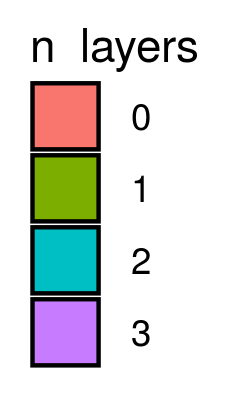
\includegraphics[width=0.75\columnwidth]{figs/sampler.png}
\end{subfigure}
\caption{On the left we display the adversarial loss (the accuracy of the adversary on $c$) and predictive accurracy on $y$ for three methods, plus the majority-class baseline, on both Adult and German datasets. For \textbf{adv. loss lower is better}, while for \textbf{pred. acc. higher is better}. On the right we plot adversarial loss by varying adversarial strength (indicated by color), parameterized by the number of layers from zero (logistic regression) to three. All evaluations are performed on the hold-out test sets.}\label{fig:pred_acc}
\end{center}
\end{figure}

% \begin{figure}[htb]
% \begin{center}
% \centering
% 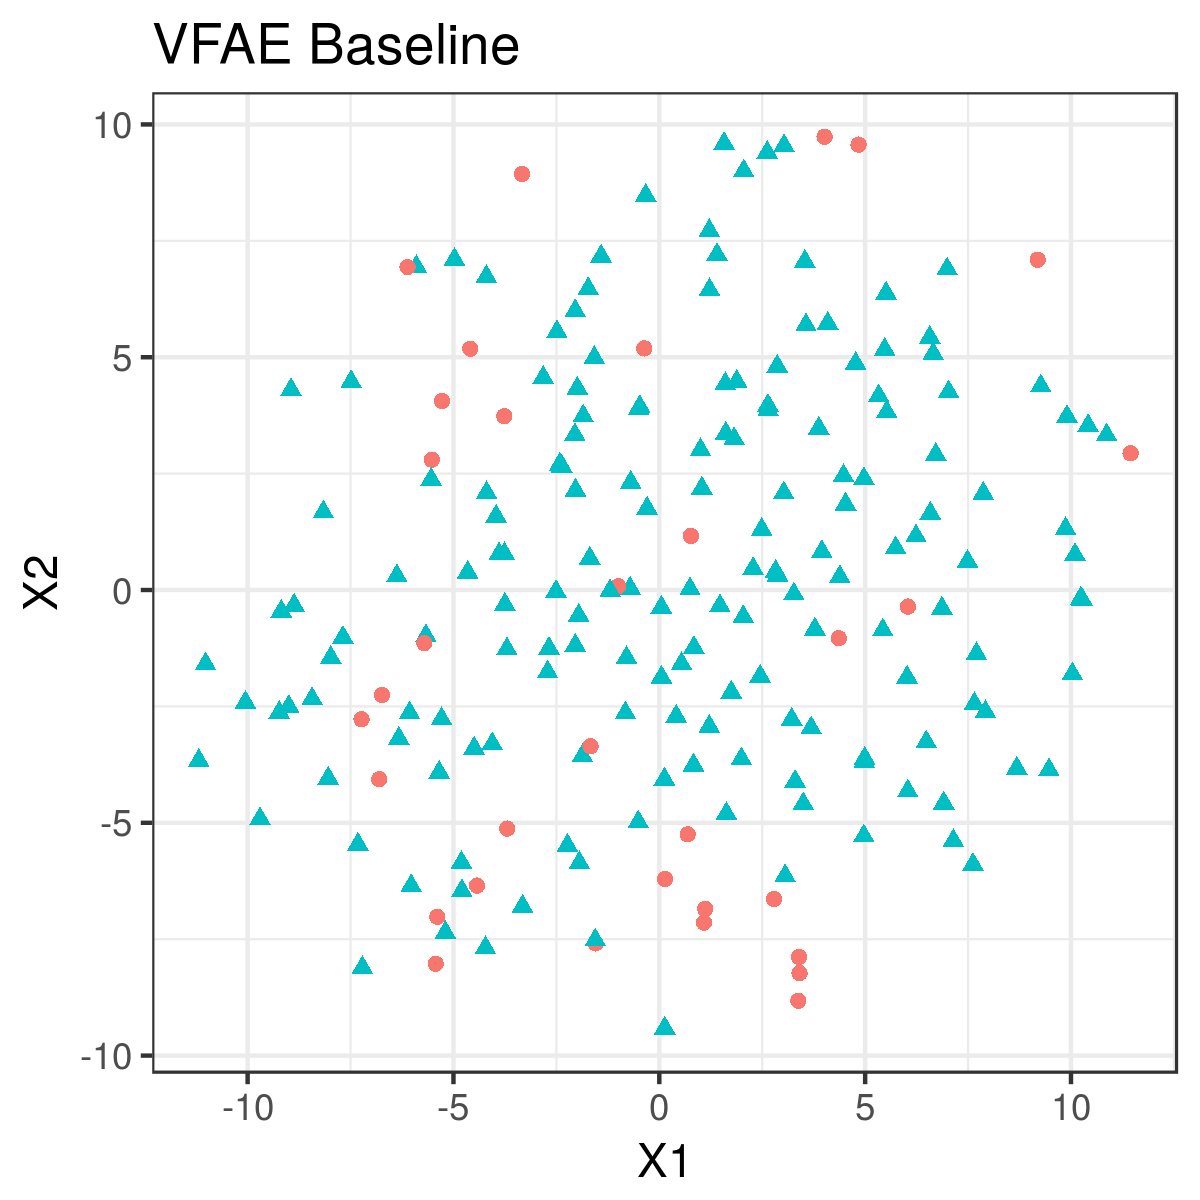
\includegraphics[width=0.3\columnwidth]{figs/bvfae_german.png}
% 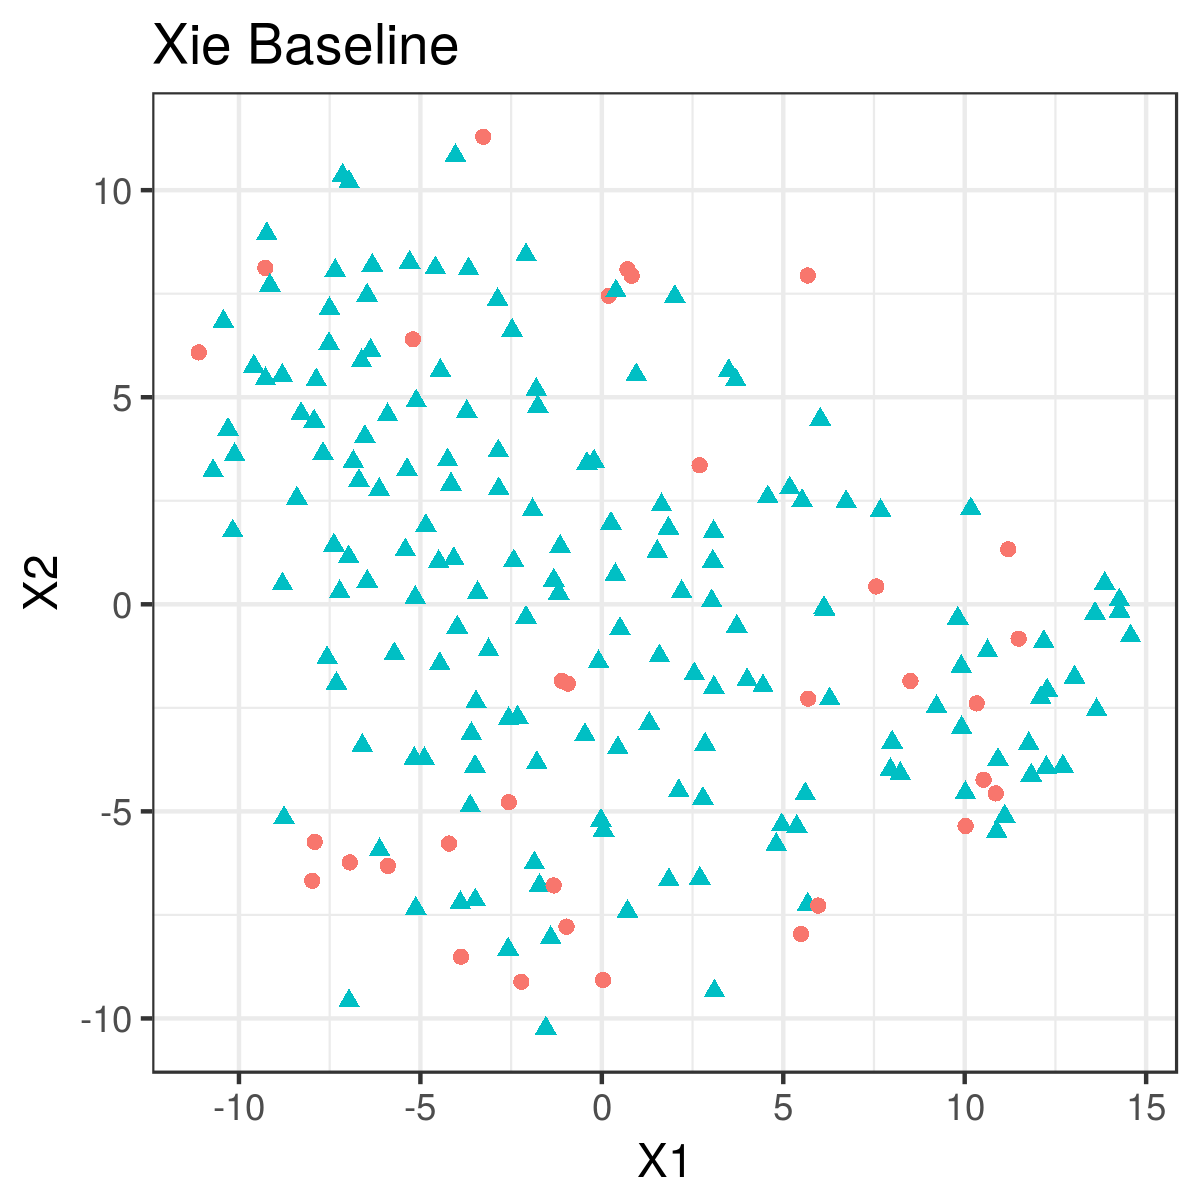
\includegraphics[width=0.3\columnwidth]{figs/xie_german.png}
% 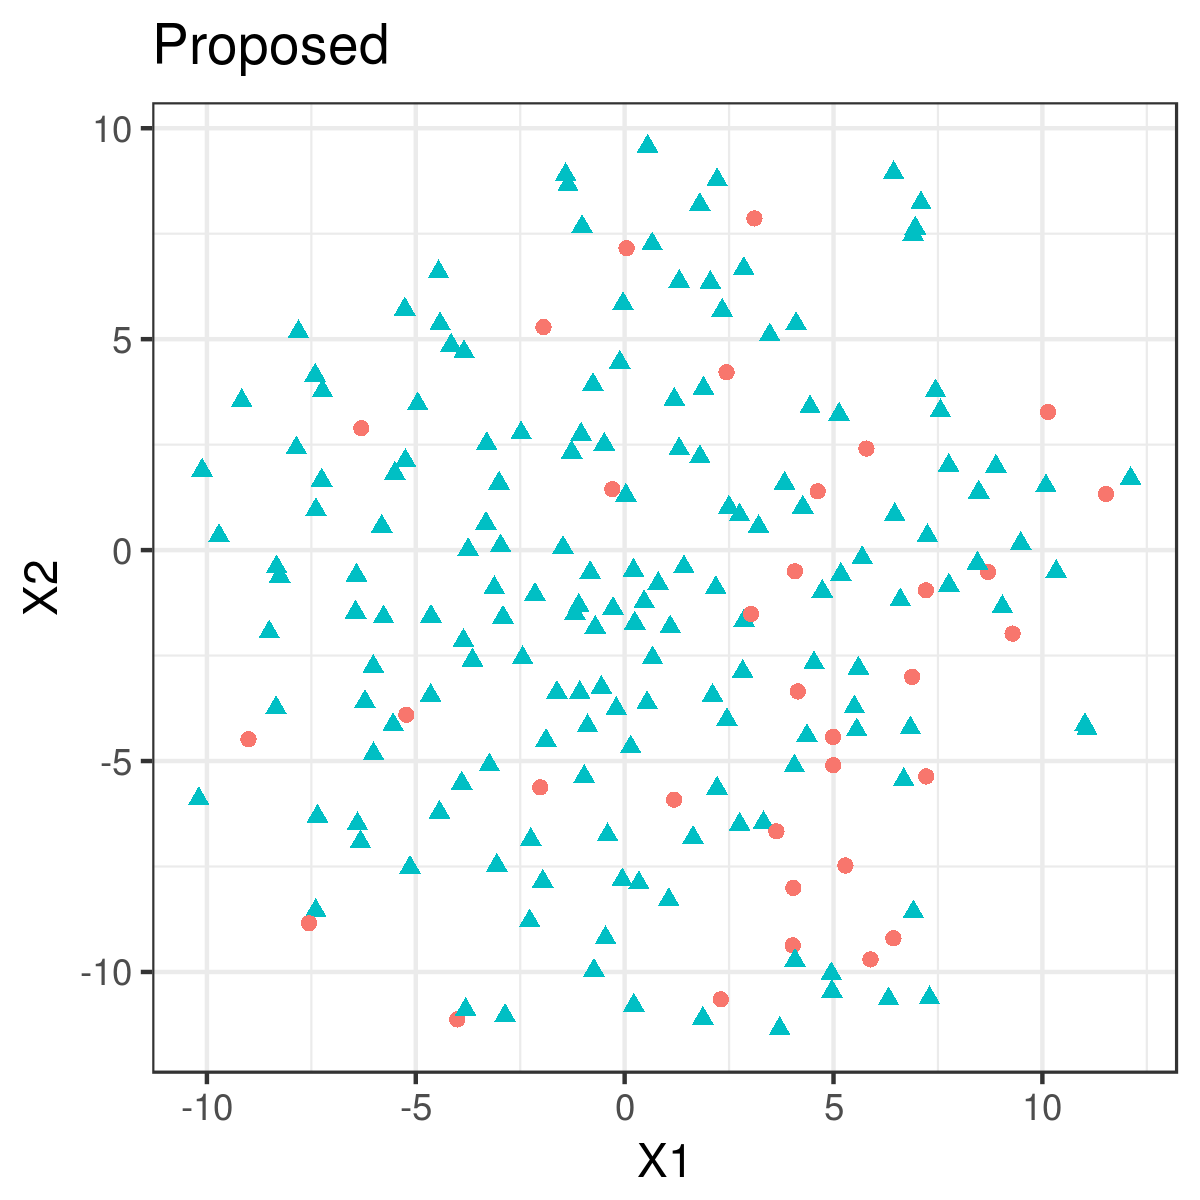
\includegraphics[width=0.3\columnwidth]{figs/navib_german.png}

% \caption{t-SNE plots for the latent encodings of (Right to Left) the VFAE, Xie et al., and our proposed method on the German dataset.}\label{fig:vae_mnist}
% \end{center}
% \end{figure}

\begin{figure}[t]
\begin{center}
\centering

\includegraphics[width=0.3\columnwidth]{new_figs/bvfae_adult.png}

\includegraphics[width=0.3\columnwidth]{new_figs/xie_adult.png}

\includegraphics[width=0.3\columnwidth]{new_figs/new_new_figs/navib_adult.png}

\caption{t-SNE plots for the latent encodings of (Left to Right) the VFAE, Xie et al., and our proposed method on the Adult dataset (first 1000 pts., test split). The value of the $c$ variable is provided as color, where {\color{graph_orred} red} is the majority class.}\label{fig:err}
\end{center}
\end{figure}

\begin{figure}[htb]
\begin{center}
\centering
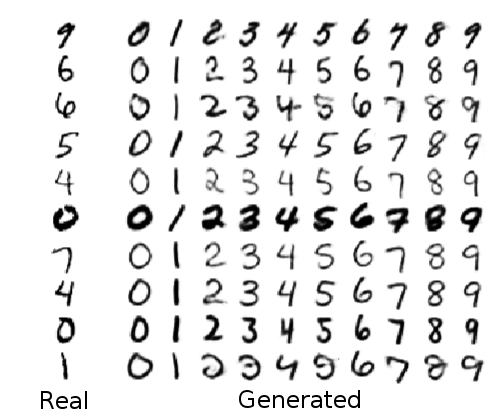
\includegraphics[width=0.8\columnwidth]{figs/vae_mnist.png}
\caption{We demonstrate the ability to generate stylistically similar images of varying classes using the MNIST dataset. The left column is mapped into $z$ that is invariant to its digit label $c$. We then can generate an image using $z$ and any other specified digit, $c'$, as show on the right.}\label{fig:vae_mnist}
\end{center}
\end{figure}

For the German dataset shown on top table of Figure \ref{fig:pred_acc}, the methods are roughly equivalent. All methods have comparable predictive accuracy, while the VFAE and the proposed method have competitive adversarial loss. In general however, the smaller dataset does not differentiate the methods.

For the larger Adult dataset shown on the bottom table of Figure \ref{fig:pred_acc}, all three methods again have comparable predictive accuracy. However, against stronger adversaries each baseline has very high loss. Our proposed method has comparable accuracy with the VFAE, while providing the best adversarial error across all four adversarial difficulty levels.

We further visualized a projection of the latent codes $z$ using t-SNE \cite{maaten2008visualizing}; invariant representations should produce inseparable embeddings for each class. All methods have large red-only regions; this is somewhat expected for the majority class. However, both baseline methods have blue-only regions, while the proposed method has only a heterogenous region\footnote{Previous versions of this paper had severely contorted latent codes for the Xie et al. baseline. Further investigation showed this to be a convergence issue. Mild performance improvements were also observed.}.

Figure \ref{fig:vae_mnist} demonstrates our ability to manipulate the conditional decoder. The left column contain the actual images (randomly selected from the test set), while the right columns contain images generated using the decoder.  Particularly notable are the transfer of azimuth and thickness, and the failure of some styles to transfer to some digits (usually curved to straight digits or vice versa).

%Both VFAE and our proposed method have relatively round distributions; this may be due to the Gaussian parametrization used. Xie et al. instead has a multi-armed distribution, with clear clusters corresponding to one label or the other. VFAE appears still to be separable, while our proposed method is well mixed.
